\documentclass[14pt,a4paper]{article}
\usepackage[latin1]{inputenc}
\usepackage[T1]{fontenc}
\usepackage[english]{babel}
\usepackage{amsmath}
\usepackage{amsfonts}
\usepackage{amssymb}
\usepackage{makeidx}
\usepackage{amsthm}
\usepackage{geometry}
\usepackage[linesnumbered,ruled]{algorithm2e}
\usepackage{tikz}
\usetikzlibrary{automata, positioning}
\usepackage{float}
\usepackage[round]{natbib}
\usepackage[hidelinks]{hyperref}
\usepackage{caption}
\usepackage{graphicx}
\usepackage{subcaption}
\usepackage{listings}
\usepackage{color}
\usepackage{ dsfont }
\usepackage[justification=centering]{caption}
\usepackage{eqnarray}
\usepackage{blindtext}
\usepackage{csquotes}

\makeatletter
\@addtoreset{section}{part}
\makeatother  


\let\oldpart\part
\renewcommand\part{\newpage\oldpart}

\def\code#1{\texttt{#1}}
\newtheorem{theorem}{Theorem}[section]
\def\iff{\Leftrightarrow}
\theoremstyle{definition}
\newtheorem{madef}{Definition}[section]
\newtheorem{prop}{Proposition}[section]
\newtheorem*{remark}{Remark}

 
\definecolor{codegreen}{rgb}{0,0.6,0}
\definecolor{codegray}{rgb}{0.5,0.5,0.5}
\definecolor{codepurple}{rgb}{0.58,0,0.82}
\definecolor{backcolour}{rgb}{0.95,0.95,0.92}

\lstdefinestyle{mystyle}{
    backgroundcolor=\color{backcolour},   
    commentstyle=\color{codegreen},
    keywordstyle=\color{magenta},
    numberstyle=\tiny\color{codegray},
    stringstyle=\color{codepurple},
    basicstyle=\footnotesize,
    breakatwhitespace=false,         
    breaklines=true,                 
    captionpos=b,                    
    keepspaces=true,                 
    numbers=left,                    
    numbersep=5pt,                  
    showspaces=false,                
    showstringspaces=false,
    showtabs=false,                  
    tabsize=2
}
 
\lstset{style=mystyle}



%to hide the todos or to show them
%\usepackage[colorinlistoftodos,prependcaption,obeyDraft]{todonotes}
\usepackage[colorinlistoftodos,prependcaption]{todonotes}


\usepackage{xargs}                      % Use more than one optional parameter in a new commands
\newcommandx{\unsure}[2][1=]{\todo[linecolor=red,backgroundcolor=red!65,bordercolor=red,#1]{#2}}
\newcommandx{\change}[2][1=]{\todo[linecolor=blue,backgroundcolor=blue!25,bordercolor=blue,#1]{#2}}
\newcommandx{\info}[2][1=]{\todo[linecolor=OliveGreen,backgroundcolor=OliveGreen!25,bordercolor=OliveGreen,#1]{#2}}
\newcommandx{\improvement}[2][1=]{\todo[linecolor=Plum,backgroundcolor=Plum!25,bordercolor=Plum,#1]{#2}}
\newcommandx{\idea}[2][1=]{\todo[linecolor=green,backgroundcolor=green!25,bordercolor=green,#1]{#2}}



\numberwithin{equation}{subsection}

%\oddsidemargin  0in
%\evensidemargin  0in
%\textwidth   6.3in
%\textheight  9.5in
%\topmargin  -0.7in


\usepackage{fancyhdr}


\author{Charles Dufour}
\title{Bachelor Project: \\
Reinforcement learning and robot navigation}
\begin{document}

\begin{titlepage}
\newcommand{\HRule}{\rule{\linewidth}{0.5mm}} % Defines a new command for the horizontal lines, change thickness here

\center % Center everything on the page
 
%----------------------------------------------------------------------------------------
%   HEADING SECTIONS
%----------------------------------------------------------------------------------------

\vspace{3cm}
\textsc{\LARGE \'Ecole polytechnique f\'ed\'erale de Lausanne}\\[0.5cm] % Name of your university/college
\textsc{\large Disopt}\\[1.5cm] % Name of your university/college
\textsc{\LARGE Master semester project}\\[0.5cm] % Major heading such as course name
\textsc{\large Autumn Semester 2019 }\\[0.5cm] % Minor heading such as course title

%----------------------------------------------------------------------------------------
%   TITLE SECTION
%----------------------------------------------------------------------------------------

\HRule \\[0.4cm]
{ \huge \bfseries A combinatorial approach to the trains routing problem}\\[0.4cm] % Title of your document
\HRule \\[1.5cm]
 
%----------------------------------------------------------------------------------------
%   AUTHOR SECTION
%----------------------------------------------------------------------------------------

\begin{minipage}{0.4\textwidth}
\begin{flushleft} \large
\emph{Student:}\\
Charles Dufour
\end{flushleft}
\end{minipage}
~
\begin{minipage}{0.4\textwidth}
\begin{flushright} \large
\emph{Supervisors:} \\
Prof. Friedrich Eisenbrand \\% Supervisor's Name
Jonas Racine
\end{flushright}
\end{minipage}\\[5cm]

%----------------------------------------------------------------------------------------
%   LOGO SECTION
%----------------------------------------------------------------------------------------
\centering
 
\includegraphics[width=0.5\linewidth]{img/logo.eps}\\ % Include a department/university logo - this will require the graphicx package

 
 
%----------------------------------------------------------------------------------------

\vfill % Fill the rest of the page with whitespace


\end{titlepage}

%\thispagestyle{empty}
%\clearpage\null



\newpage
\pagestyle{fancy}
%\lfoot{Charles DUFOUR}
%\rfoot{\today}
%\fancyhead[R]{}
\fancyhead[L]{}




\tableofcontents
\pagenumbering{gobble}

\newpage


%\thispagestyle{empty}
%\clearpage\null\newpage






\pagenumbering{arabic}
\section*{Introduction}
\label{sec:intro}
\addcontentsline{toc}{section}{\nameref{sec:intro}}

$\quad$ We tackle the \emph{vehicle routing problem (VRP)} and \emph{vehicle re-scheduling problem (VRSP)} through an online competition. We first develop a particular graph to model the underlying railway network. We then formulate our problem as a \emph{dynamic minimum cost multicommodity flow problem}, and derive the explicit column generation method to solve it efficiently.

All the code can be found in this repository (\cite{GIT}).





\section{Flatland Challenge}
\todo[inline]{\blindtext \\ \blindtext}




\newpage
\section{Modelization of the environment}

To have a formulation of our problem in term of dynamic multicommodity flows (\emph{multicommodity flows over time}), we need to first define the graph representing the railway network from the 2D grid world. Then we need to embed the time component in our model using a time expanded network, bringing our problem back to a static multicommodity flow problem.
We first model the problem with a unique speed for all trains.

\subsection{Transition network}

We create a graph to model all the possible switches and rails in the rail network from Flatland. In order to do so, we model each cell as a super node containing 8 internal nodes, as can be seen in Figure \ref{fig:simple_super_node}. These internal nodes are responsible for correctly implementing the different transitions the original cell allows. 


\begin{figure}[h]
	\begin{minipage}{0.5\linewidth}
	\centering
	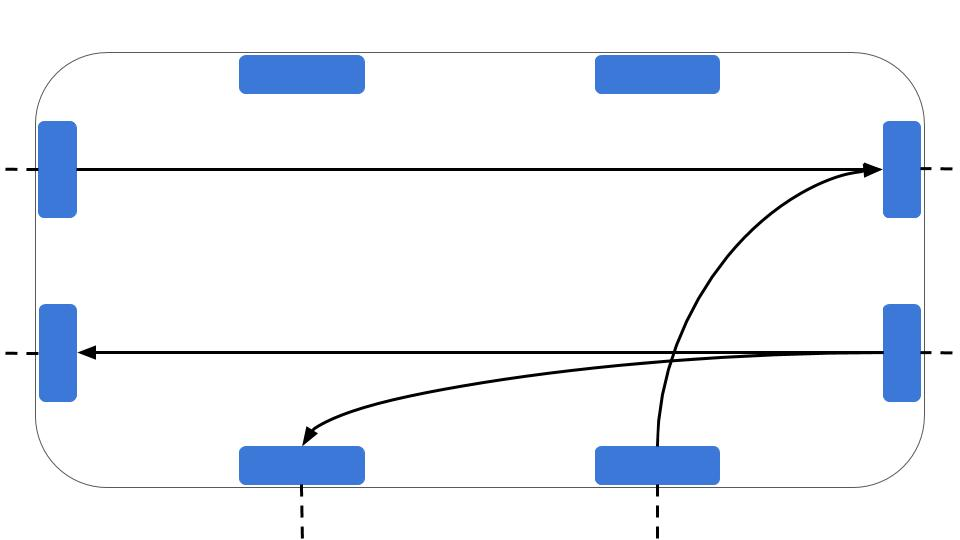
\includegraphics[width=0.9\linewidth]{img/super_node.jpg}
	\caption{Super node representing the cell represented in Figure \ref{fig:cell super node example}. The blue rectangles represent the internal nodes of the cell, where the big white rectangle represents the super node.}
	\label{fig:simple_super_node}
	\end{minipage}
	\begin{minipage}{0.5\linewidth}
	\centering
	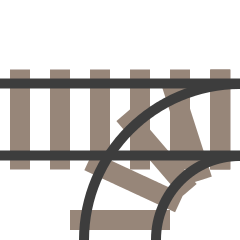
\includegraphics[width=0.5\linewidth]{img/switch.png}
	\caption{A switch from the railway network.}
	\vspace{1.6cm}
	\label{fig:cell super node example}
	\end{minipage}
\end{figure}

The transition network is an oriented graph $G = (V,A)$ that represents the original 2D grid world. Figure \ref{fig:both} shows an example of a randomly generated environment and its corresponding transition graph.

\begin{figure}[h]
	\begin{minipage}{0.3\linewidth}
		
		
		
		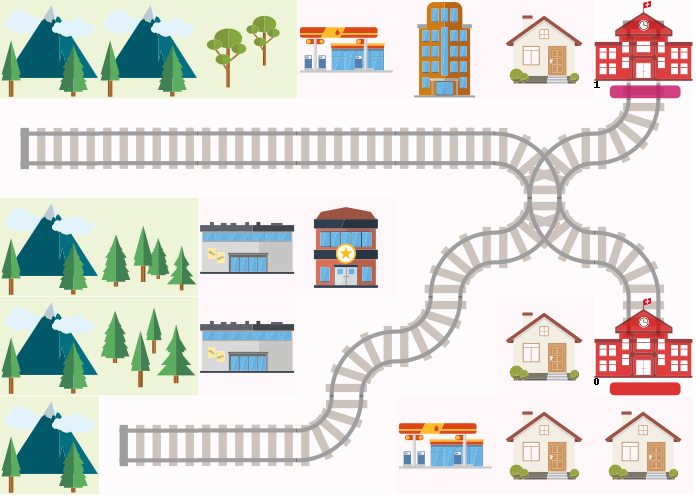
\includegraphics[width=\linewidth]{img/env.png}
		\caption*{Flatland environment.}
		\label{fig:env}
	\end{minipage}
	\begin{minipage}{0.6\linewidth}
		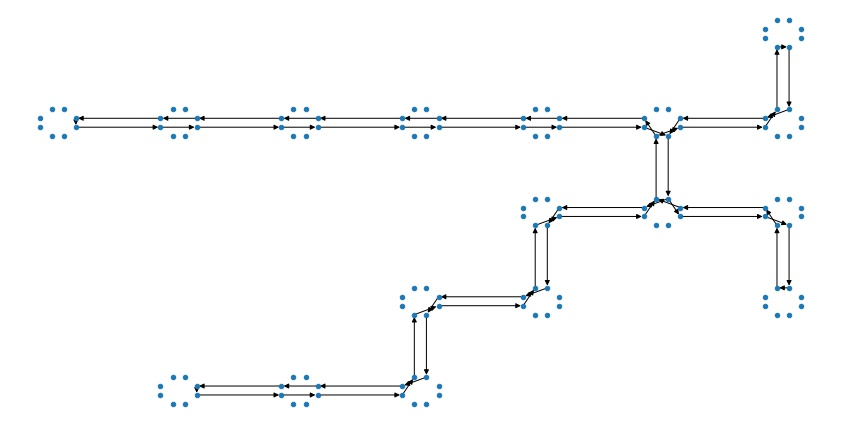
\includegraphics[width=\linewidth]{img/env_graph.jpg}
		\caption*{Transition graph.}
	\end{minipage}
	\caption{Randomly generated $7 \times 5$ grid and its extracted transition graph.}
	\label{fig:both}
\end{figure}


Why did we not use a single node to represent each cell and connect it to its neighbors if there is a connection between them? The problem with the simple node modelization is that it allows transition that are not represented in the original railway network. Take for example the switch in Figure \ref{fig:cell super node example}: with a simple node representation, a train coming from a cell below could go to the left whereas in the original cell it should not be possible.
\newline

There exists alternatives to model railway networks, namely the double vertex graphs (see for example the modelization done in  \cite{BachelorThesis}). Those were not considered here since they are not simple directed graphs. Indeed they have a particular definition of paths, so the usual flows algorithm would not be straightforward to apply.





\subsection{Time expanded network}
\label{ten}

We now have to include the time component in our design. We will use a time expanded network to bring back our dynamic multicommodity flow problem to a static formulation. 

Intuitively we define a discrete time step (given by the environment in our case) and a maximum time horizon $T$. Now we do $T$ copies of the nodes of our graph, and only allow transition from one time step to another. Figure \ref{fig:ten intuition} shows the intuition by drawing a path in a time expanded network.


\begin{figure}[h]
	\centering
	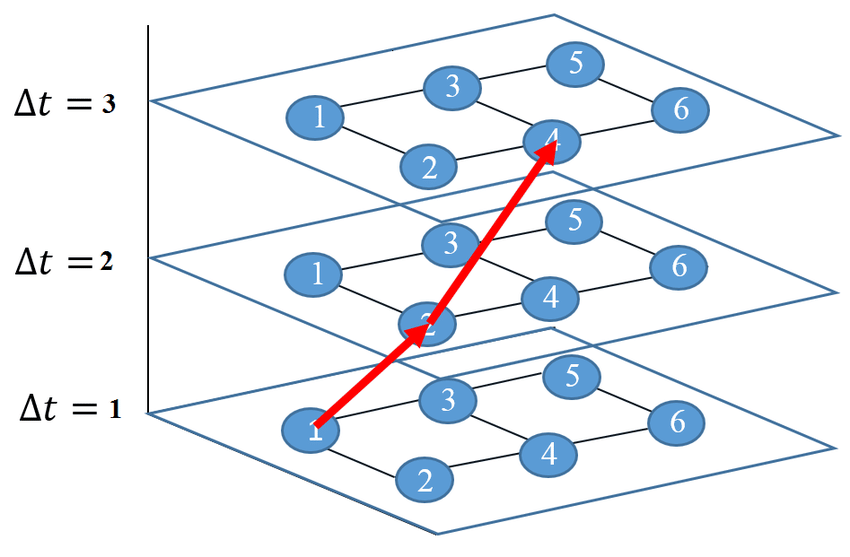
\includegraphics[width=0.6\linewidth]{img/Example-of-links-in-a-time-expanded-network.png}
	\caption{Explanation of the intuition of time expanded networks with only the path $\{1,2,4\}$ drawn in time (image from \cite{TENExample}).}
	\label{fig:ten intuition}
\end{figure}


We now give a formal definition from \cite[p.~19]{Skutella2008AnIT}:
\begin{madef}[Time-expanded network]
	 Let $G = (V, E)$ be a network with capacities $u$ and costs $c$ on the arcs. For a given time horizon $T\in \mathds{Z}_{>0}$ ,	the corresponding \emph{time-expanded network} $G^T = (V^T, E^T)$ with capacities and costs on the arcs
	is defined as follows. For each node $v\in V$ we create $T$ copies $v_0 , v_1 , \ldots, v_{T-1} $, that is,
	$$V^T := \{v_\theta | v \in V, \theta = 0, 1, \ldots, T-1\}.$$
	For each arc $e = (v, w) \in E$, there are $T-1$  copies $e_0,e_1,\ldots,e_{T-2}$ where arc $e_\theta$ connects
	node $v_\theta$ to node $w_{\theta+1}$ . Arc $e_\theta$ has capacity $u_{e_{\theta}}:= u_{e}$ and cost $c_{e_{\theta}}:= c_{e}$. Moreover, $E^T$ contains
	\emph{waiting} arcs $(v_\theta , v _{\theta+1})$ for $v \in V$ and $\theta = 0,\ldots, T-2$. The capacity of waiting arcs is $1$
	and they have cost $1$. Summarizing, the set of arcs $E^T$ is given by
	\begin{align*}
	 E^T := &\{e_\theta = (v_\theta,w_{\theta+1})| e = (u,v) \in E, \theta=0,1,\ldots,T-2 \} \\
	 &\cup \{(v_\theta,v_{\theta+1})|v\in V, \theta=0,1,\ldots,T-2 \}
	 \end{align*}
\end{madef}

Notice that the size of the	time-expanded network $G^T$ is linear in $T$ and therefore only pseudo-polynomial in the input size.




We then proceed to define a time step, which represent what would be added to a time expanded graph, were we to expand the horizon by one.

\begin{madef}[Time step in time expanded network]	
	A \emph{time step} at time $\theta$ is the set of all edges $(v_\theta,w)$ for all $v \in V$, $w \in V^T$ such that $(v_\theta,w) \in E^T$. 
	It represents the set of all edges starting at time $\theta$.
\end{madef}


\begin{remark}
	There are no cycles in the time expanded network since $\nexists (v_\theta,w_{\tilde{\theta}}) \in E^T$ with $\tilde{\theta} < \theta$.
\end{remark}
	
\subsection{Restrictions}
\label{sec:restrictions}
In the environment from Flatland some position are forbidden: two trains cannot be at the same cell at the same time, and to trains can collide, meaning they cannot swap positions.  We will first define the restrictions needed on the transition network and then explain how to impose the same restriction on the time expansion of this network.

A restriction will impose that among a certain set of edges, only one of them can be used at the same time.

\subsubsection{On the transition network}



\begin{itemize}
	\item Position constraint\\
	All the edges leading to specific supernode should be \emph{restricted}. Using these restrictions, we ensure that at any time step, at most one train will be in any cell, thus avoiding collisions.
	\item Swapping constraint
	All pairs of edges between two supernodes shouls be \emph{restricted}. It is trivial to see that these restrictions will be enough to prevent swapping.
\end{itemize}


\begin{figure}[h]
	\centering
	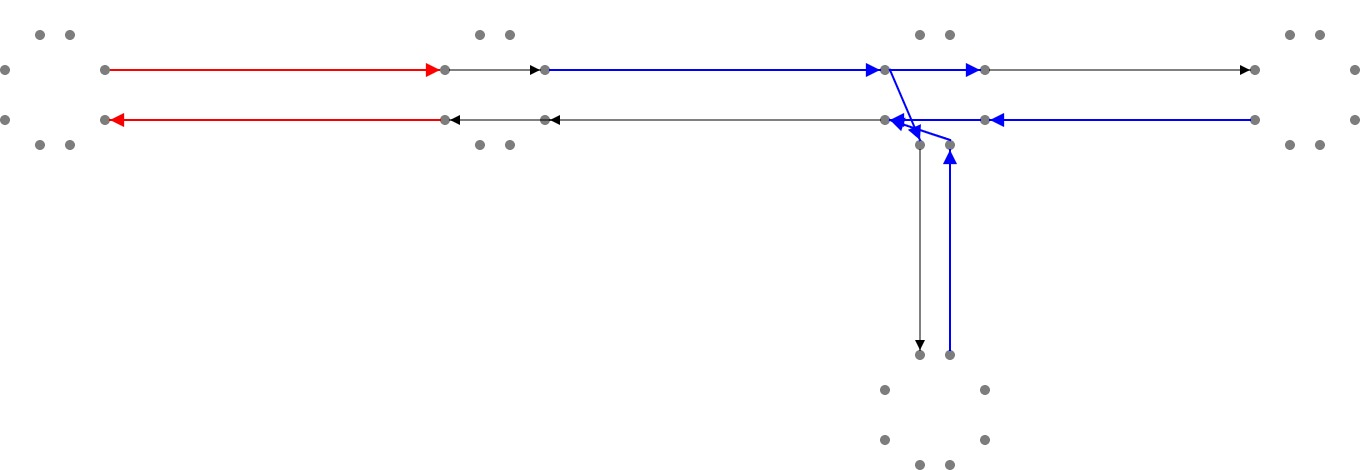
\includegraphics[width=0.9\linewidth]{img/rail_split_edge.jpg}
	\caption{Representation of some restrictions in the transition network. All the edges colored in the same color (blue or red) cannot be used at the same time. The blue edges represent a position restriction and the red edges a swapping restriction. }
	\label{fig:restrictions}
\end{figure}

\subsubsection{On the time expanded network}
\label{restrictions}

The restrictions on the time expanded network can be easily derived from the restrictions described before. Suppose we have a restriction on  $\left\{(u,v),(i,j)\right\}$. In the time expanded network, we will have restrictions for all sets $\left\{(u_{t},v_{t+1}),(i_{t},j_{t+1})\right\} \ \forall t \in \{1,\ldots,T-1\}$. 

We also have to add to the position constraints the waiting edges. Let's say we consider a cell $i$ with its corresponding supernode, all the waiting edges of this supernode should be added to the position constraint linked to cell $i$.

\begin{remark}
	Due to the nature of the restrictions, a path in the time expanded network can only take one edge per restriction. Indeed, otherwise it would mean that at a certain time $t$, the path takes two edges in the transition network at the same time which is impossible.
\end{remark}



\subsection{Dealing with different train speeds and stochastic events}

For now, the trains were supposed to all have the same speed and there were supposed to be no changes in the underlying railway network over time. This is not realistic, so in order to have a better model, we discuss now what could be implemented to handle a system with multiple speeds and random breakdown of trains.


\subsubsection{Different speeds}

In the Flatland challenge, trains can have different speeds. The speeds will be defined as follow. The faster trains will have a speed of $1$, meaning that it takes them one time step to go between two nodes in the transition graph. Then all the other train will have a speed $v \in [0,1]$ with $v$ representing the percentage of the edge that is traveled by said train in one time step. For example, if a train a speed $1/3$, it will take 3 time steps to travel through an edge.

Now suppose we have only two different speeds (the discussion easily generalize to $k$ different speeds), namely $1$ and $v$ (w.l.o.g. we say that one of the two speeds is $1$ otherwise we would just rescale all of them).

We can then build two time expanded networks, one for each speed. The tricky parts are the restrictions: they now span the two networks. Indeed, now one train takes $v^-1$ time steps to go through an edge, while the other takes only one time step, so it is necessary to have the constraints spanning the 2 networks.


The way to do it is to have the fastest train's network as a point of reference. This one has the usual constraints, to which we had edges from the other graph. Take a constraint, and look at the edges contained in it. You then take the corresponding edges (representing the same railway piece), and add them for the corresponding time steps.

\begin{figure}[h]
	\centering
	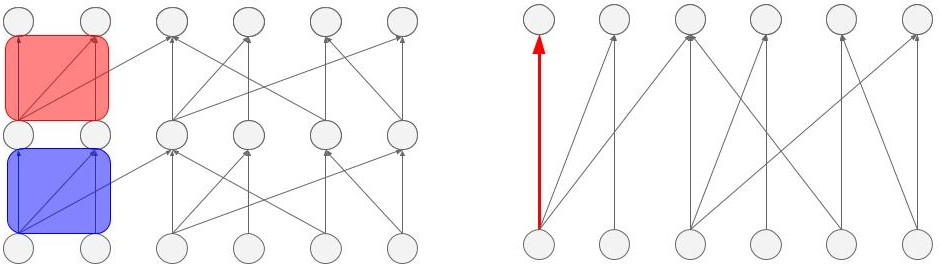
\includegraphics[width=0.7\linewidth]{img/ten_constraints_multiple_constraints.jpg}
	\caption{On the left the fast expanded network, on the right the slow ($v = 0.5$). The red edges on the right will belong to both the red and blue restrictions showed on the left (fictional restriction sets).}
	\label{fig:multiple constraints}
\end{figure} 

For example if the second speed was $0.5$, we would have edges $(u_0,v_1)$,$(u_1,v_2)$ in the fast time expanded network, and only $(u_0,v_2)$ in the slow network. For the restriction containing $(u_0,v_1)$ we would have to add $(u_0,v_2)$ and the same for the one containing $(u_1,v_2)$. Figure \ref{fig:multiple constraints} shows this.




A formal way to say this would be that for any edge $(u_{t1},v_{t2})'$ in the slow network it has to be added to any constraint from the fast network $(u_t,v_{t+1})$ if $t1\geq t$ and $t2 \leq t+1$.
\newline


One could argue about building only one network combining the edges of our two networks. The reason we build two different network is for efficiency when finding minimum weighted path during the column generation pricing problem (see subsection \ref{pricing}).

\subsubsection{Stochastic events}



In the case of failure in the network, there will be  unusable tracks (cells) for a certain period of time (known or unknown depending on the setting). In this case one can still use our method.
When a failure happens, suppose $k$ trains break down among the $n$ in the network. The cells occupied by the broken trains will be unusable for a certain period of time $T$. We now propose multiple approaches.
\begin{itemize}



		\item Restart from scratch all the trains, taking as initial position their position at failure time. When the trains are reactivated (failure is resolved) solve once more to move all the trains to their destination.
		\item Reroute only the trains affected by the failure in a modified time expanded network

\end{itemize}




The following sections considers one unique speed for all the trains and no stochastic events. This can easily be adapted  following the above discussion.
\newpage
\section{Minimum cost multicommodity flow}

We now consider the time expanded network defined in section \ref*{ten} and denote it by $G = (V,A)$. The trains will be the commodities, we suppose that we have $K$ of them.

We now formalize the definition of restriction as described in section \ref*{sec:restrictions}.

\begin{madef}
	A restriction $R$ over a time expanded network $G = (V,A)$ is a set of arcs: $R \subset A$ over which we want to impose certains specification (e.g. global capacity).
	
	We define $C_R$ the set of all restrictions over the time expanded network $G$.
\end{madef}



We also introduce a notation:
\begin{madef}
	Given $\alpha$ a set,
	\[
	\delta_\alpha(\beta)=\left\{
	\begin{array}{ll}
	 \mathds{1}{\{\beta \cap \alpha \neq \emptyset\}} \text{ if } \beta \text{ is a set}\\
	\mathds{1}{\{\beta \in \alpha\}} \text{ otherwise}\\
	\end{array}
	\right.
	\]
	Informally this represents the fact that $\alpha$ and $\beta$ are not disjoint or that $\beta$ is contained in $\alpha$.

\end{madef}


\subsection{Arc flow formulation}

The minimum cost multicommodity flow can be formulate as an arc-flow integer program: 

\begin{equation}
\begin{array}{ll@{}ll}
\text{minimize}  & \displaystyle\sum\limits_{k=1}^{K}\sum_{(i,j)\in A} x_{ij}^k &\\
\text{subject to}& \displaystyle\sum\limits_{k=1}^{K}   x_{ij}^k \leq 1,  &\forall (i,j) \in A \\
& \displaystyle\sum\limits_{k=1}^{K}\sum_{(i,j) \in R}   x_{ij}^k \leq 1, \quad \quad  &\forall R \in C_R \\
& Nx^k = b^k,  &\forall k \in \{1,\ldots,K\}\\
&                                                x_{ij}^k \in \{0,1\}, & \forall (i,j)\in A
\end{array}
\label{eq:arcFlow}
\end{equation}

Where $N^k$ is the -arc adjacency matrix, and $b^k$ is such that 
\[
b^k_i=\left\{
\begin{array}{ll}
1 \text{ if node } i \text{ is a source for commodity } k\\
-1 \text{ if node } i \text{ is a sink for commodity } k\\
0 \text{ otherwise}\\
\end{array}
\right.
\]



This formulation is clear and intuitive: for each commodity we decide whether or not it will use a specific arc at a certain time by setting $x_{ij}^k$ to $1$ or to $0$. But this formulation \eqref{eq:arcFlow} is not scalable due to its high number of restrictions and variables (see section \ref{results:arcsVSflow} for a more detailed explanation). We then proceed to find new ways to solve this problem.









\subsection{Column generation method}

In this section, we give a column generation solution procedure that works with arbitrary restrictions, as long as the restrictions do not span more than one time step (see section \ref*{sec:restrictions} for an explanation). We directly consider the relaxation problem.

\subsubsection{Reformulation as a path flow problem}


For this section we will restate our problem using path flows instead of arc flows as before. In this paradigm, we suppose that we list all the possible paths between the sources and targets, $\mathcal{P}$. Then for each path $P \in \mathcal{P}$ we decide how much we send along this path with the variable $f(P)$.


 The problem then becomes: 
\begin{equation}
	\begin{array}{ll@{}ll}
		\text{minimize}  & \displaystyle\sum\limits_{P \in \mathcal{P}} &f(P)|P| &\\
		\text{subject to}& \displaystyle\sum\limits_{P \in \mathcal{P}_R}   &f(P) \leq 1,  &\forall R \in C_R\\
	& \displaystyle\sum\limits_{P \in P^k}   &f(P) = 1,  &\forall k \in \{1,\ldots,K\}\\
		&                                                &f(P) \geq 0, &P\in \mathcal{P}
	\end{array}
\label{eq:pathFormulationPrimal}
\end{equation}

With: 
\begin{itemize}
	\item $\mathcal{P} = \{\mathcal{P}_1,\ldots,\mathcal{P}_K\}$ and $\mathcal{P}_i$ is all the possible distinct paths between $s_i$ and $t_i$.
	\item $\mathcal{P}_R = {P \in \mathcal{P}: |P\cap R| > 0 }$. This represents the paths that "goes trough" the restriction $R$.
\end{itemize}

The second restriction $\sum_{P \in P^k} f(P) = 1$ contains in our case the fact that we need to have exactly one train going from $s_k$ to $t_k$ for each commodity.


The dual of the primal formulation (\ref{eq:pathFormulationPrimal}) is:

\begin{equation}
\begin{array}{ll@{}lll}
\text{maximize}  &\displaystyle\sum\limits_{R \in C_R} &y_R  +\displaystyle\sum\limits_{i=1}^{K}\sigma_i &\\
\text{subject to}  & \displaystyle\sum\limits_{R \in C_R}   &\delta_P(R)\cdot y_R + \sigma_k \leq |P|,  &\forall P \in \mathcal{P}\\
 &                                               &y \leq 0, &y \in \mathbb{R}^{|C_R|} \\
 &												 & &\sigma \in \mathbb{R}^K\\
\end{array}
\label{eq:pathFormulationDual}
\end{equation}




With respect of the dual variables,the reduced cost $c_P^{\sigma,y}$ for each path flow variable $f(P)$ which belongs to commodity $k$ is :
\begin{equation}
 c_P^{\sigma,y} = |P| - \sum\limits_{R \in C_R}   \delta_P(R)\cdot y_R -\sigma_k
\label{eq:reducedCost}
\end{equation}


We can then derive complementary slackness conditions.

\begin{theorem}[Path flow complementary slackness conditions]
	The commodity pah flow $f(P)$ are optimal in the path flow formulation \eqref{eq:pathFormulationPrimal} of the multicommodity flow problem if and only if for some restriction prices $y_R$ and commodity prices $\sigma_k$, the reduced cost and arc flows satisfy the following complementary slackness conditions: 
	\begin{flalign}
	&y_R\left[\displaystyle\sum_{k\in [K]}\sum_{P\in P^k} \delta_P(R)\cdot f(P) - 1\right]= 0 \text{ for all } R \in C_R. \label{eq:cond1}\\
	&c_P^{\sigma,y} \geq 0 \text{ for all } k \in [K] \text{ and all }P \in P^k. \label{eq:cond2}\\
	&c_P^{\sigma,y}\cdot f(P) = 0 \text{ for all k } \in [K] \text{ and all } P\in P^k. \label{eq:cond3}
	\end{flalign}
	\label{theorem:slackcond}
\end{theorem}


\begin{proof}[Proof of theorem \ref{theorem:slackcond}]$ $\\
	 We show that optimality of the primal \eqref{eq:pathFormulationPrimal} implies the complementarity slackness conditions from theorem \ref{theorem:slackcond}. 
	 
	 Denote $f^*(\mathcal{P}),y^*_{S}$ and $\sigma^*_k$ the optimal solution from \eqref{eq:pathFormulationPrimal} and \eqref{eq:pathFormulationDual}. Since $y^*$ and $\sigma^*$ are solution of the dual formulation we get condition \eqref{eq:cond2} directly.
	 
	 To show the other two conditions, we will write the primal and dual expression in matrix form.
	 
	 \paragraph{Primal}
	 \begin{equation*}
	 	\begin{array}{ll@{}ll}
	 \text{minimize}  &b^T f(\mathcal{P})  \\
	 \\
	 \text{subject to} 
	 &\left( \begin{matrix} -A_{C_R}	\\ A_K \\ -A_K \\ \end{matrix} \right) \cdot f(\mathcal{P}) \geq  \left( \begin{matrix} -1_{|C_R|}	\\ 1_K \\ -1_K \\ \end{matrix} \right) \\
	 \\
	                                          &f(\mathcal{P}) \geq 0
	 \end{array}
	 \label{eq:matrixformprimal}
	 \end{equation*}
	 
	 With: 
	 \begin{itemize}
	 	\item $b \in \mathbb{R}^{|\mathcal{P}|}, \quad b_P = |P|$ is the vector containing the length of the paths.
	 	\item $A_{C_R} \in \mathbb{R}^{|C_R|\times |\mathcal{P}|}$ where $\left(A_{C_R}\right)_{ij}$ is $1$ if the $i^{th}$ restriction contains an edge that belongs to the $j^{th}$ path and $0$ else.
	 	\item $A_K \in \mathbb{R}^{K\times |\mathcal{P}|}$ where $\left(A_K\right)_{ij}$ is $1$ if the $j^{th}$ path belongs to $\mathcal{P}_i$ (i.e. belongs to the $i^{th}$ commodity) and $0$ else.
	 \end{itemize}
 
 

 
 \paragraph{Dual}
 \begin{equation*}
 \begin{array}{ll@{}ll}
 \text{maximize}  &\left( \begin{matrix} -1_{|C_R|}^T, 1_K^T, -1_K^T  \end{matrix} \right)\cdot \tilde{y}   \\
 \\
 \text{subject to} 
 &\left( \begin{matrix} -A_{C_R}^T, A_K^T, -A_K^T \end{matrix} \right) \cdot \tilde{y} \leq  b  \\
 \\
 &\tilde{y} \geq 0
 \end{array}
 \label{eq:matrixformdual}
 \end{equation*}
 
 Where $\tilde{y} =\left( \begin{matrix} -y \\ \tilde{\sigma_1} \\ \tilde{\sigma_2}  \end{matrix} \right) $ with $y \in \mathbb{R}^{|C_R|}$  and $\tilde{\sigma_1} + \tilde{\sigma_2} = \sigma \in \mathbb{R}^{K}$, with $y,\sigma$ being as \eqref{eq:pathFormulationDual}.

 
 Then we rewrite the conditions \eqref{eq:cond1} and \eqref{eq:cond3} in matrix form:
\begin{align*}
&\left[ \left( \left( \begin{matrix} -1_{|C_R|}^T, 1_K^T, -1_K^T  \end{matrix} \right) - f(\mathcal{P})^T\left( \begin{matrix} -A_{C_R}^T, A_K^T, -A_K^T \end{matrix} \right) \right) \cdot \tilde{y}\right]_{i}= 0 & \text{ for all } i \in \{0,1\ldots,|C_R| \}\\
& f(\mathcal{P})^T\left( b - \left( \begin{matrix} -A_{C_R}^T, A_K^T, -A_K^T \end{matrix} \right)\tilde{y} \right) = 0 &
\end{align*}
 
 
 By the weak duality theorem we have: 
 $$\left( \begin{matrix} -1_{|C_R|}^T, 1_K^T, -1_K^T  \end{matrix} \right)\cdot \tilde{y} \leq  
 f(\mathcal{P})^T \left( \begin{matrix} -A_{C_R}^T, A_K^T, -A_K^T \end{matrix} \right)\tilde{y} \leq f(\mathcal{P})^Tb $$
 
 Using the strong duality theorem, we also have 
 $$\left( \begin{matrix} -1_{|C_R|}^T, 1_K^T, -1_K^T  \end{matrix} \right)\cdot \tilde{y} =  f(\mathcal{P})^Tb  $$

Combining the two results from strong an weak duality we get the following two equalities:
\begin{align*}
\left( \begin{matrix} -1_{|C_R|}^T, 1_K^T, -1_K^T  \end{matrix} \right)\cdot \tilde{y} = 
f(\mathcal{P})^T \left( \begin{matrix} -A_{C_R}^T, A_K^T, -A_K^T \end{matrix} \right)\tilde{y} \\
f(\mathcal{P})^T \left( \begin{matrix} -A_{C_R}^T, A_K^T, -A_K^T \end{matrix} \right)\tilde{y} =  f(\mathcal{P})^Tb 
\end{align*}

Which is exactly what we aimed to obtain.

The other direction is similar.

	 
	 
\end{proof}
\subsubsection{Column generation method}

For each train, we will only use one path in the time expanded network, so even if the path formulation \eqref{eq:pathFormulationPrimal} leads to an exponential number of variables, actually only $K$ of them will be useful in the end. 

With this remark in mind, the purpose of the column generation method is to gradually improve a feasible solution containing few variables until we have the optimal solution. The idea is that in a few iterations we should be able to find the optimal solution, leading us to consider a small number of variables compared to all the possible paths set. See \cite{LectureNotes} for a more in depth explanation of the column generation method.
\\

We define the restricted linear program on a basis (set of variables) as the linear program \eqref{eq:pathFormulationPrimal} setting all variables at $0$ except for the variable contained in the basis.\\



\begin{algorithm}[H]
	\SetAlgoLined
	\KwResult{Optimal solution to \eqref{eq:pathFormulationPrimal}}
	\KwIn{Basis: initial feasible solution}

	\While{solution optimal}{
	Solve restricted linear program on the basis\;
	Solve the pricing problem to find useful variables to add\;
	Add these variables to the basis\;
	}

	Return solution of restricted linear program on the basis\;
	
	
	\caption{Column generation algorithm}
\end{algorithm}






\paragraph{Pricing problem}
\label{pricing}

Following \cite[p.~669]{networkflows}, we consider only \eqref{eq:cond2}. Indeed for any basis use for the restricted linear program, the conditions \eqref{eq:cond1} and \eqref{eq:cond3} are automatically respected. One can see this by explicitly deriving the dual variables from the restricted primal, and see that $c_P^{\sigma,w} = 0 ~\forall p$ in the basis $\mathcal{B}$ and $y_R = 0$  if $\nexists p \in \mathcal{B}$ st $\delta_P(R) = 1$ (the restriction is not used by the basis).\\

 The only indication of the basis not being optimal is then the second condition \eqref{eq:cond2}.If we find a path with a negative reduced cost, we can add it to the basis and improve our actual cost. We see now that the pricing problem can be efficiently solved.
 
\newpage
\paragraph{Solving the pricing problem efficiently}
Because of the particular nature of the restrictions in our problem, one can see that no restriction can span more than one time step in the time expanded network, and that a path cannot have two edges in the same time step (see section \ref*{restrictions}). 

Based on these observations, we define the cost of an arc in the graph as:
\begin{equation*}
w_{ij} = -\sum_{R \in C_R} \delta_R((i,j))\cdot y_R \geq 0
\end{equation*}

One can notice that 
$$ \sum_{(i,j)\in P}\left(\sum_{R \in C_R} \delta_R((i,j))\cdot y_R \right)=   \sum\limits_{R \in C_R}    \delta_P(R)\cdot y_R$$



We can then rewrite the reduced cost as: 
$$ c_P^{\sigma,y} = |P| + \sum\limits_{(i,j) \in P}  w_{ij} -\sigma_k $$

So equation \eqref{eq:cond2} becomes:

\begin{eqnarray*}
		c_P^{\sigma,y} & \geq 0 &\forall P \in P^k\\
		|P| + \sum\limits_{(i,j) \in P}  w_{ij} -\sigma_k & \geq 0 &\forall P \in P^k\\
		|P| + \sum\limits_{(i,j) \in P}  w_{ij}  & \geq \sigma_k &\forall P \in P^k\\
		\sum\limits_{(i,j) \in P} \left( w_{ij} + 1\right)  & \geq \sigma_k &\forall P \in P^k\\
		\min_{P\in P^k}\sum\limits_{(i,j) \in P} \left( w_{ij} + 1\right)  & \geq \sigma_k & \\
\end{eqnarray*}



This shows that the pricing problem can efficiently be solved by searching for a weighted shortest paths $p^*_k$ between $s_k$ and $t_k$ for all commodities $k \in [K]$ . The weight for each arc $(i,j)\in A$ is given by $\tilde{w}_{ij} = w_{ij}+1$. We can use Dijkstra's algorithm to efficiently solve this problem since the weights of the edges are positive.





\paragraph{Initial Solution}
We produce an initial feasible solution using a greedy algorithm.\\


\begin{algorithm}[H]
	\SetAlgoLined
	\KwResult{ $\{p_1^0,\ldots,p_K^0 \}$, where $p_k^0$ is a path from $s_k$ to $t_k$}
	pathsFeasible $= [$  $]$\;
	Set weight at $1$ for all edges\;
	
	\For{$k \in \{1,\ldots,K\}$}{
		find shortest path candidate $\tilde{p}$ from $s_k$ to $t_k$ using Dijkstra's algorithm \label{shortestpath}\;
		\If{$ \tilde{p}$ does not have any conflicts with pathsFeasible}{add $\tilde{p}$ to pathsFeasible\;}
		\Else{Increase weight of all edges of $\tilde{p}$ by $1$\;
			Goto \ref{shortestpath}\;}
	}
	
	\caption{Finding and initial feasible solution for the column generation method}
\end{algorithm}

$ $\\

Where we say that a path $p^*$ does not have conflicts with a set of paths $P$ if using formulation \eqref{eq:pathFormulationPrimal} and putting all $f(p) = 1 \quad \forall p\in P \cup \{p^*\}$ all the constraints are satisfied.



\subsubsection{Relaxation and approximation}
\label{relaxation}

After having a set of optimal paths for the fractional formulation of \eqref{eq:pathFormulationPrimal} we have to get an integral solution.

For now this is done by \cite{gurobi} automatically, using branch-price-and-cut algorithms when asked to solve the restricted master problem \eqref{eq:pathFormulationPrimal} with integer variables. A good overview of the methods can be found in \cite{BranchAndCut}, even if it might be outdated by modern software.





\newpage
\section{Results}

To solve the linear programs we use the commercial solver \cite{gurobi}. To obtain the integral solution we use their optimized algorithms which might differ from what is described in section \ref{relaxation}. The rest of the implementation is in Python and can be found at \cite{GIT}.


All experiments are done with constant speeds for all the train and no stochastic events.

\label{results}
\subsection{Experimental results}
\label{results:arcsVSflow}

\subsubsection{Arc formulation}

The arc formulation proved to be efficient for very small instances of the problem (either in term of size of the grids or in term of the number of agents present). But for bigger instances, it proved inadequate: it took more than 30 minutes to guide 3 agents in a  $(30 \times 30)$ complex environment, while it took the flow formulation approximately 3 minutes.

Figure \ref{fig:numberVar} shows why the arc formulation is inefficient by showing the average number of variables for one commodity in function of the size of the instance.


\begin{figure}[h]
	\centering
	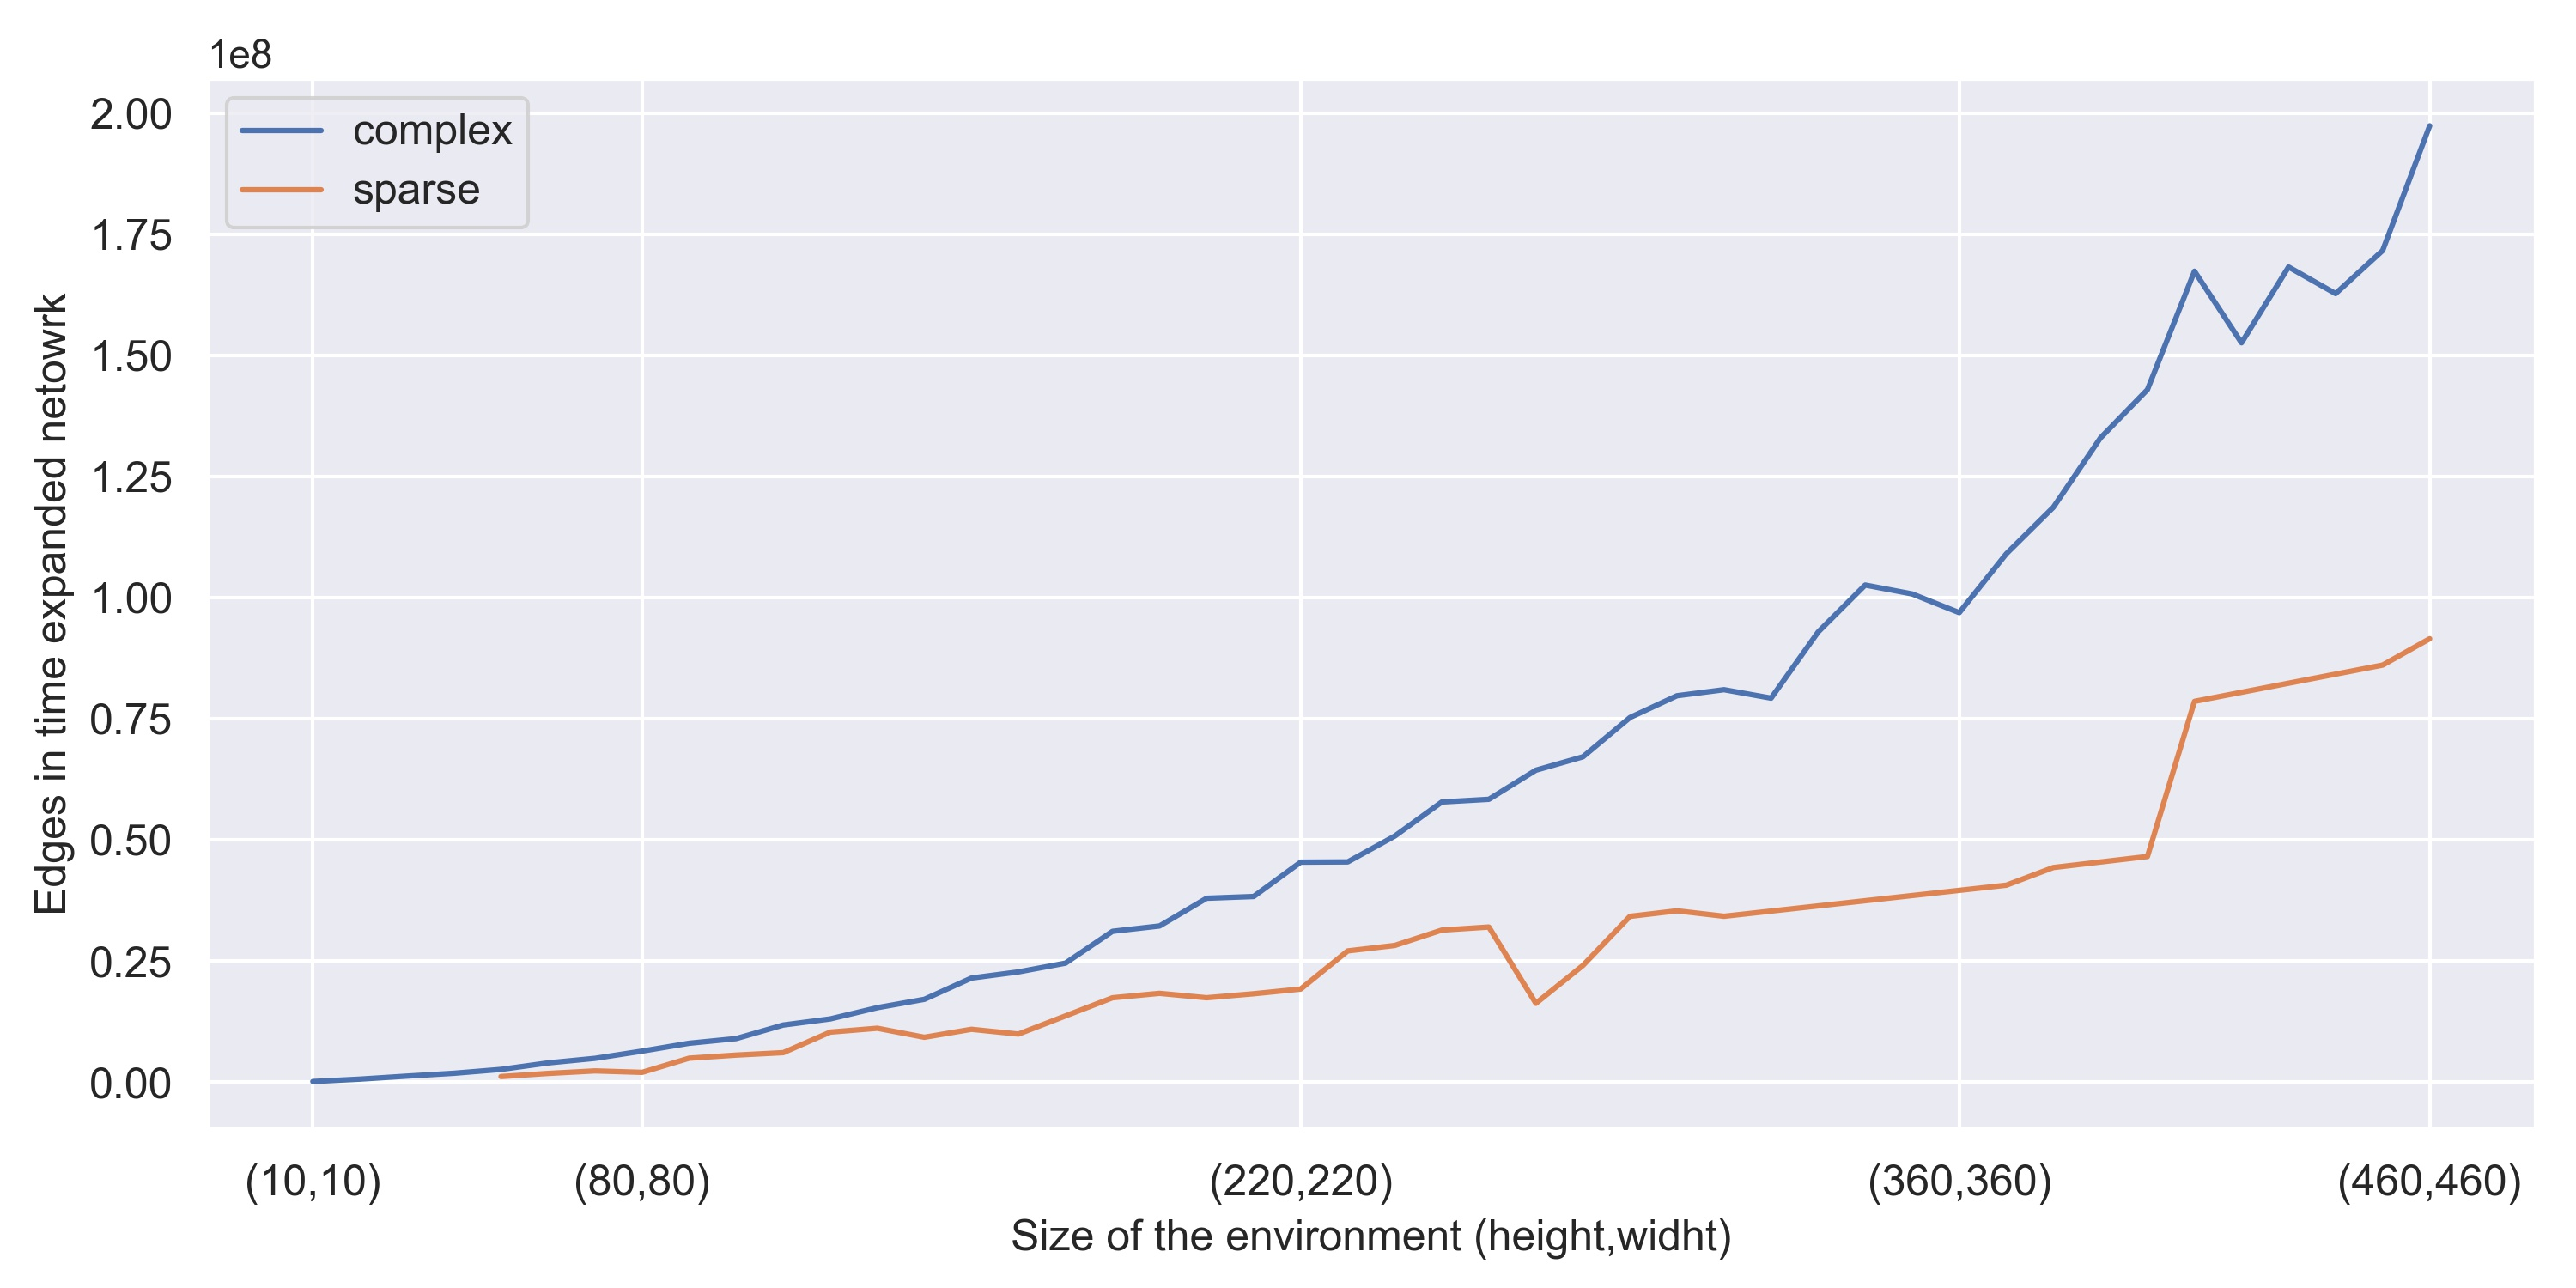
\includegraphics[width=\linewidth]{img/number_variables.jpg}
	\caption{Average number of variables in term of size of the instance (grid size of the environment).}
	\label{fig:numberVar}
\end{figure}

\subsubsection{Flow formulation}

Figure \ref{fig:time repartition} shows the time division of the solver using column generation. We see that the initial solution algorithm ends up being the bottleneck of our algorithm. \enquote{In fact, finding a feasible solution of a linear program (or a basic feasible solution) is almost as difficult as finding an optimal solution.} (\cite{networkflows}).


\begin{figure}[h]
	\centering
	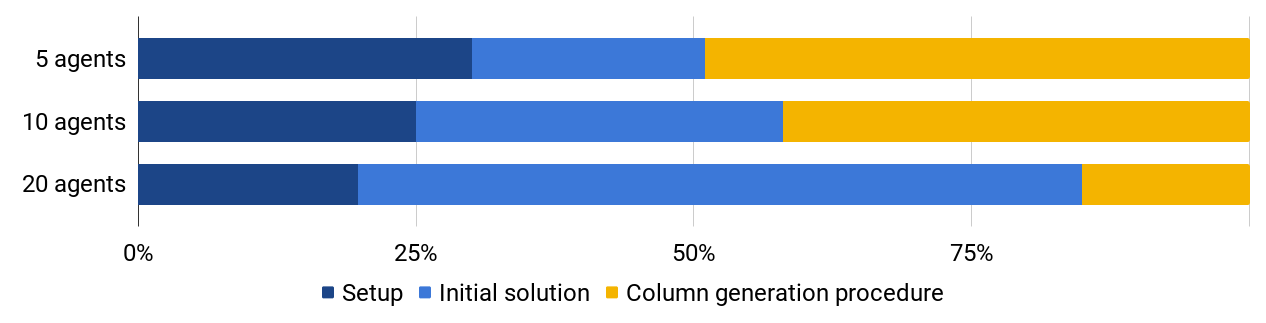
\includegraphics[width=\linewidth]{img/time_repartition.png}
	\caption{Average time division in the column generation method.}
	\label{fig:time repartition}
\end{figure}

The greedy algorithm is probably not the best way to go for this problem. Maybe trying to find first a partition of the railway network and working on each section independently would improve the initial solution algorithm.

\subsubsection{Comparison of the two formulations}

While we have seen that the number of variables for the arc formulation grows out of control even for middle-sized instance, it is interesting to note that the number of constraints in the linear program stays similar for the arc formulation and for the path formulation. Only the flow conservation constraints are lost when switching paradigm.

The two methods arrive almost always at the same cost. If there is a difference the arc formulation actually has the better solution. The difference could be explained by the way we relax our problem for the path formulation: we restrict our linear program to a set of paths that are optimal for the relaxed LP only. It is worth noting that this difference is always smaller than 2 time steps, so the flow formulation still finds very good solutions.

We now compare our two methods in term of speeds. The speed is measured from the moment the solver receives and environment from flatland to the moment it can outputs the paths for all the trains. Figure \ref{fig:comparison} shows the improvement made by the second method: we accelerate the process in average by $96\%$ for sparse environments and by $98\%$ for complex environments.

Figure \ref{fig:numberVar} explains the difference in speed gain: the sparse environment have less edges than the complex one, so the gain in reducing the number of variables is less. 

\begin{figure}[h]
	\centering
	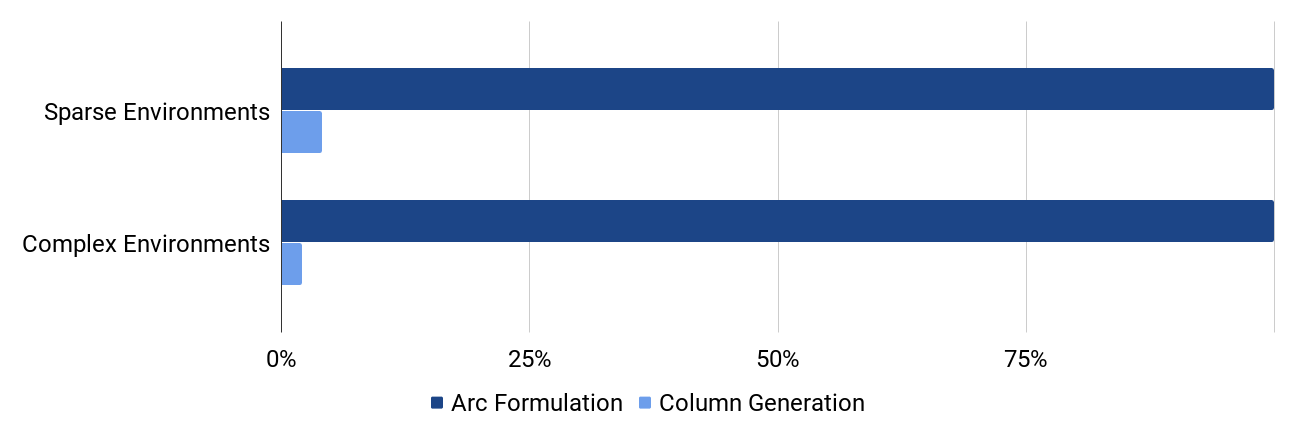
\includegraphics[width=\linewidth]{img/comparison.png}
	\caption{Comparison of the average relative speeds between the two formulation. The values were obtained by doing multiple runs on different random environments and computing the relative difference between the two methods.}
	\label{fig:comparison}
\end{figure}



\subsection{Comparison with reinforcement learning approach}

At the same time this project was made, another one was studying the use of reinforcement learning to solve this competition. Here is a brief comparison of the two, but is far from complete and should be studied much further.

We arrived at the conclusion that for the \emph{VRP}  the combinatorial approach was better in term of ease to implement and actual performance. On the other hand, considering the \emph{VRSP}, the reinforcement learning approach seems to have an edge compare to ours, due to its ability to modify trajectories \emph{on the fly}, without needing to recompute a plan for all the trains.

There is of course the difference that the reinforcement learning algorithms need days to train while the combinatorial optimization methods need none. 


\newpage
\section{On the mixed RL-CO approach}

In order to get the best of both worlds, here are our ideas on how to combine the combinatorial approach that was developed in this project with reinforcement learning.

\todo[inline]{\blindtext}





%\fancyhead[R]{\emph{CONCLUSION}}
\section*{Conclusion}
\label{sec:conclusion}
\addcontentsline{toc}{section}{\nameref{sec:conclusion}}

The \emph{vehicle routing problem (VRP)} was successfully  solved with combinatorial methods for most instances (even if for bigger instances improvements should be made). On the other hand, our formulation in term of flows failed to solve efficiently the \emph{vehicle re-scheduling problem (VRSP)} in this case.


Examples of improvements include, but are not limited to, developing a better initial solution generator, improving the data structures to minimize the memory footprint, make the solver more robust to edge cases $\ldots$ 


Other approaches such are double vertex graph (\cite{BachelorThesis}) and multiple agent path finding (MAPF) could also be considered.





\newpage
\fancyhead[R]{\emph{ANNEXES}}
\section*{Annexes}
\label{sec:annexes}
\addcontentsline{toc}{section}{\nameref{sec:annexes}}
\subsection*{Technical details about the implementation}

Here are some details of the implementation that might seem strange, or some tricks we used to try to speed up the process.
\subparagraph{Computing weights in pricing problem}
\begin{equation*}
w_{ij} = -\sum_{R \in C_R} \delta_R((i,j))\cdot y_R \geq 0
\end{equation*}

It is easier to go through the activated restrictions (i.e. restrictions through which a path of the basis is going) and add its weights on the edges belonging to this restriction. Indeed a non activated constraints will have $y_R = 0$.
\subsection*{Comparison in term of time}

\begin{figure}[h]
	\begin{minipage}{0.5\linewidth}
		
		
		
		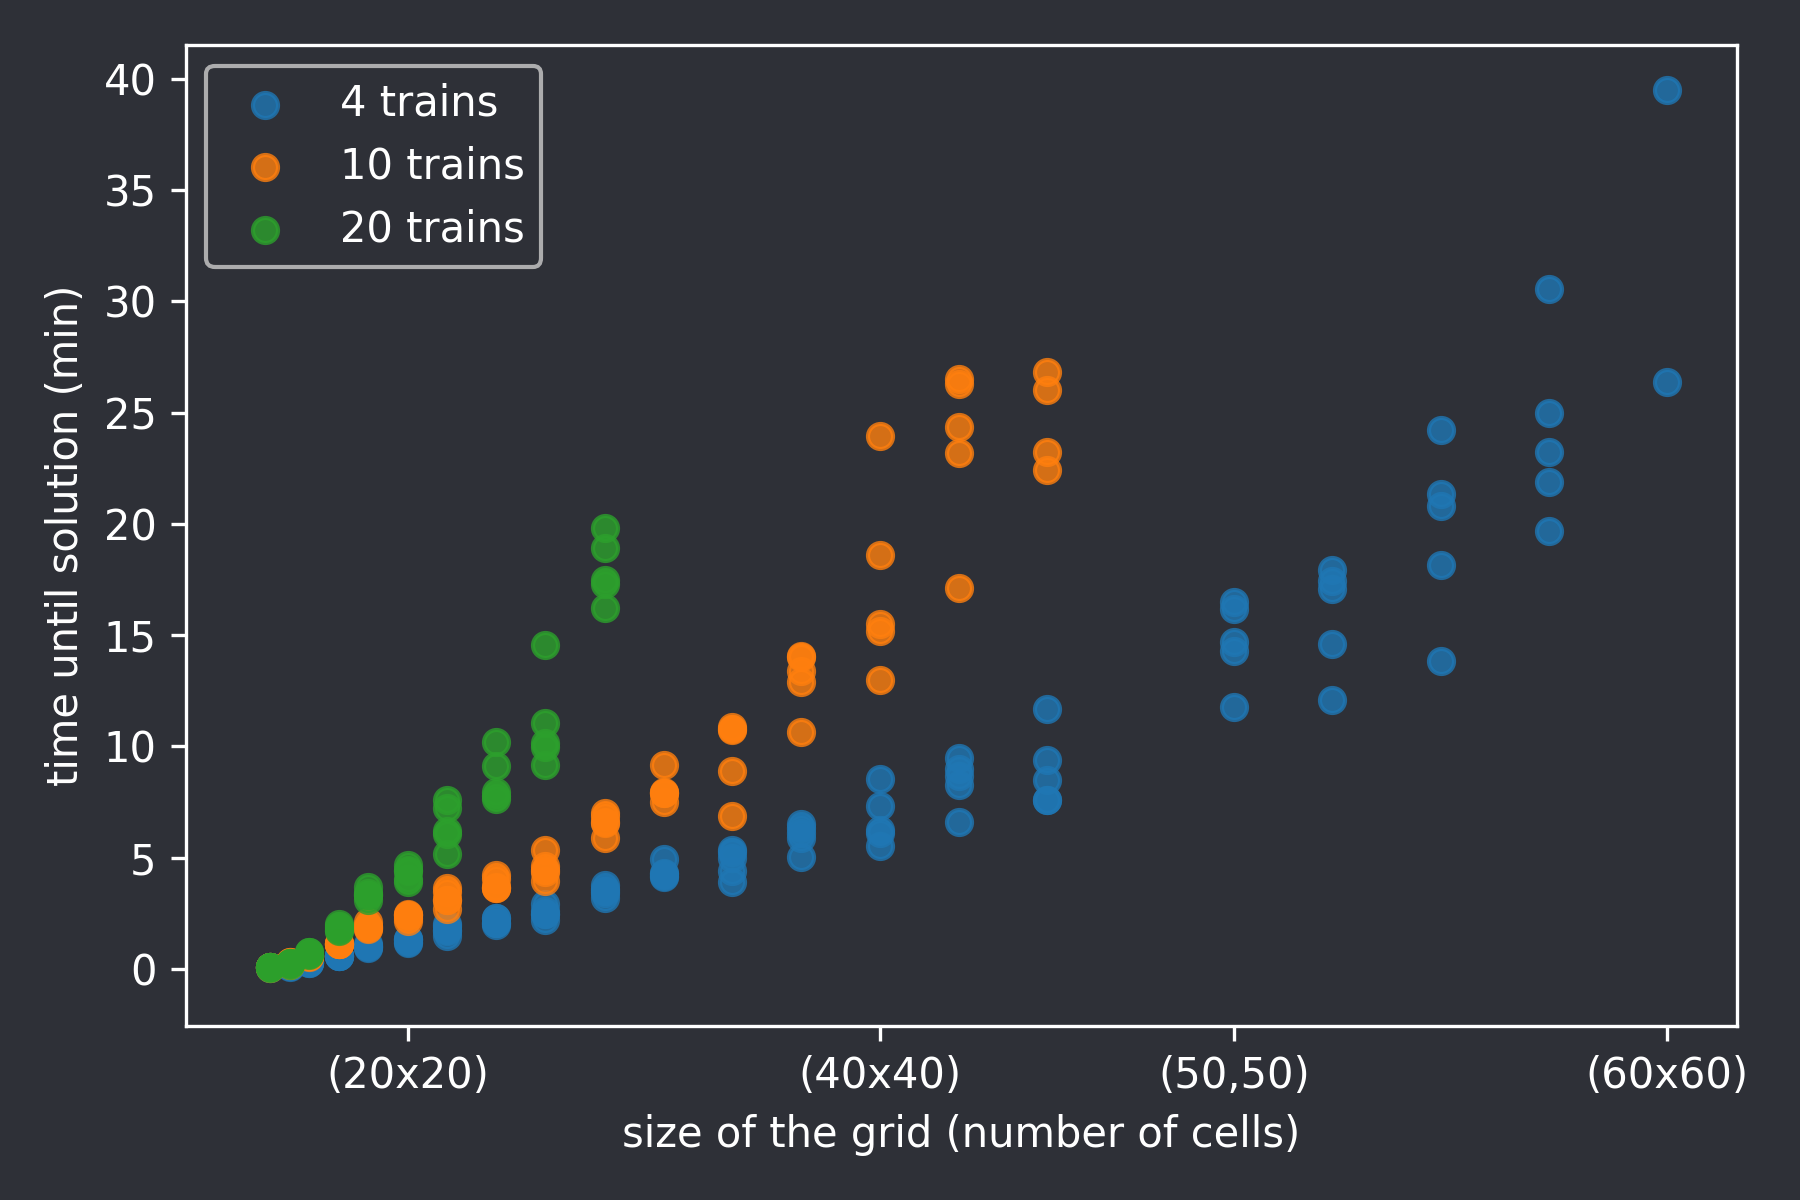
\includegraphics[width=\linewidth]{img/time1.png}
		\caption*{Arc formulation.}

	\end{minipage}
	\begin{minipage}{0.5\linewidth}
		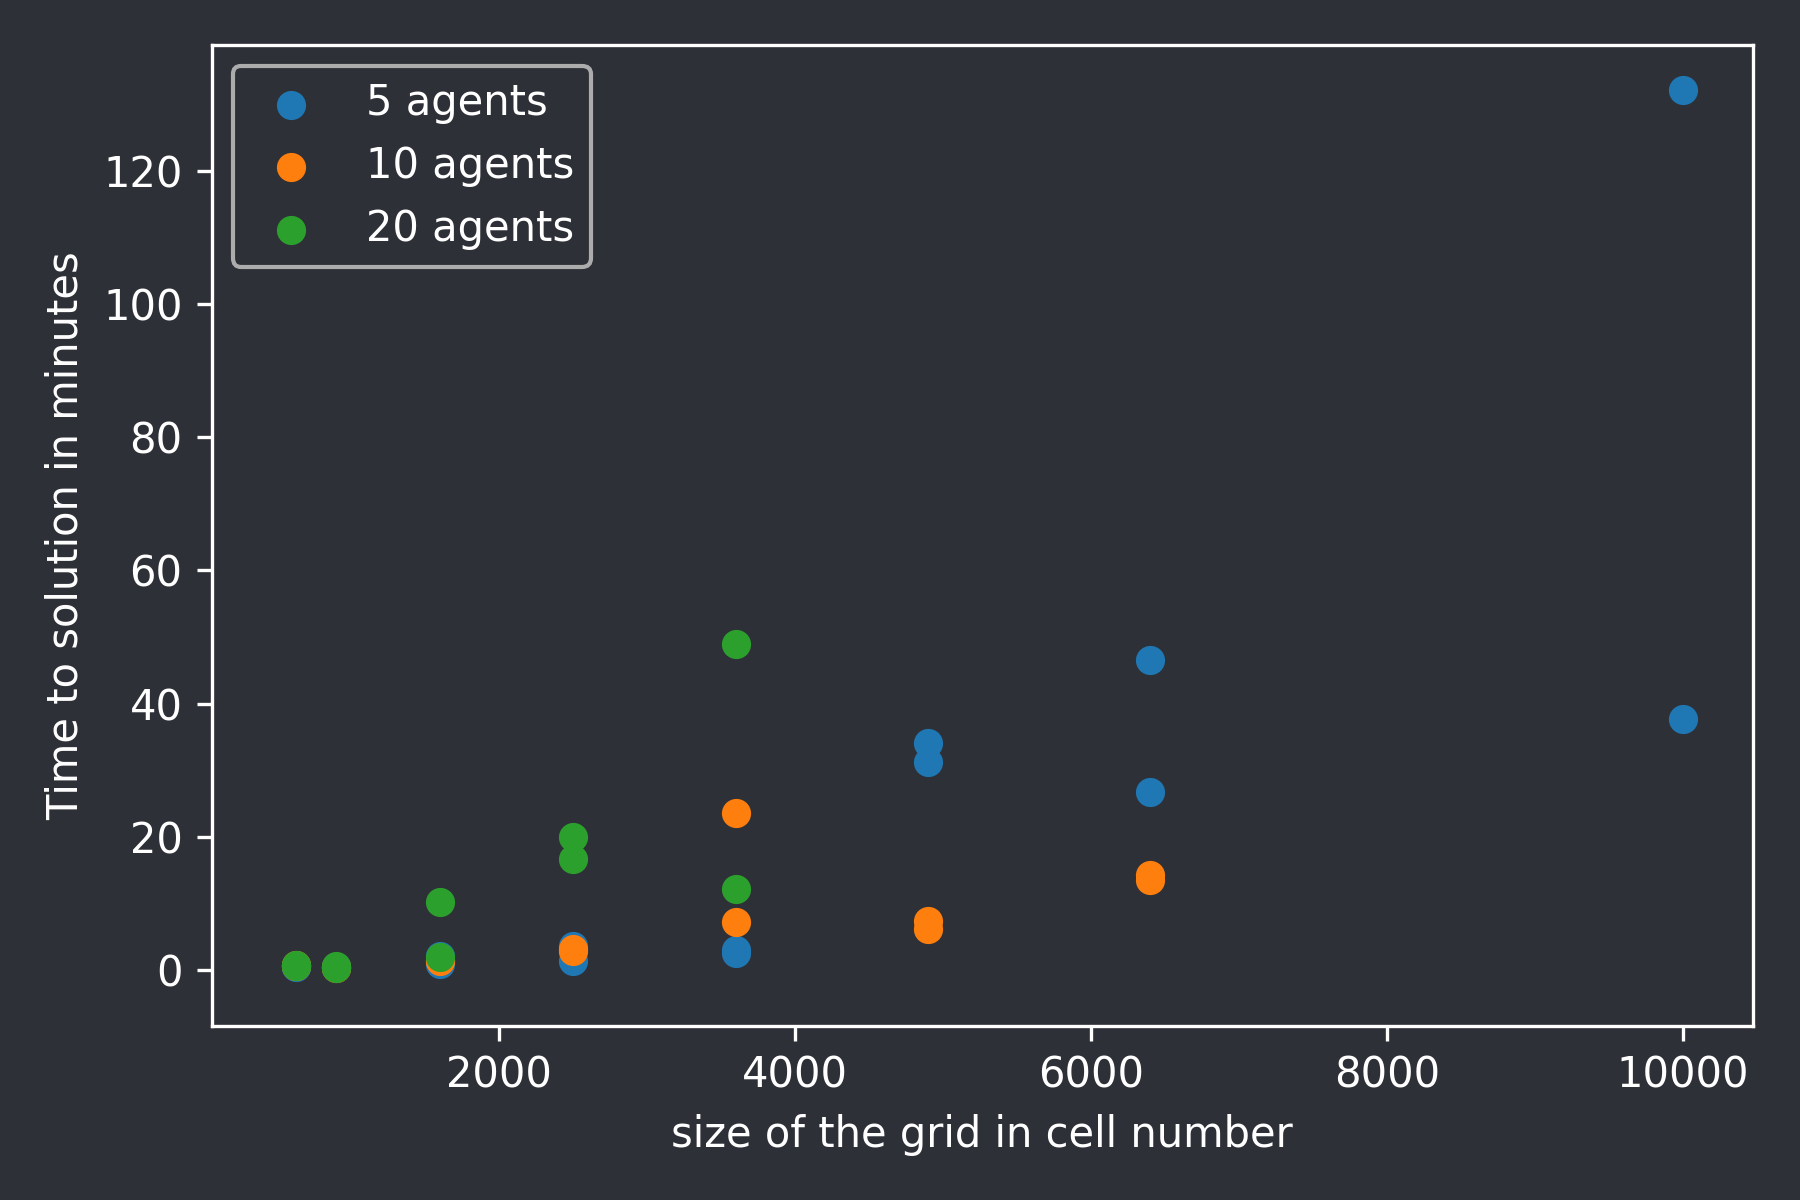
\includegraphics[width=\linewidth]{img/time2.png}
		\caption*{Column generation method.}
	\end{minipage}
	\caption{time to solution for the two combinatorial methods used, in function of the size of the grid. Beware of the change in scale in the x-axis: the graph on the right goes up to a grid of $(100\times100)$ ! }

\end{figure}



\newpage
\fancyhead[R]{\emph{REFERENCES}}
 \nocite{*} 


\bibliographystyle{apa-good}
\bibliography{ref}
\addcontentsline{toc}{section}{References}


\end{document}
